\section{Linear Relationships and the CAPM Model}
The scatter plots demonstrate a clear linear relationship between the excess returns of several stocks and the sector market
returns, particularly for Johnson \& Johnson, Pfizer, and Medtronic. 
This alignment suggests a strong correlation, with the CAPM model effectively describing the variability in their returns. 
The high $R^2$ values and significant $\beta$ coefficients observed for these stocks reinforce the reliability of the CAPM 
model in explaining their behavior. 
These findings validate the assumption that systematic risk plays a crucial role in driving stock returns within the Healthcare
sector.
The consistency of these linear relationships highlights the applicability of the CAPM framework for stocks with stable market 
exposure. 
The regression lines for these companies align closely with the observed data points, indicating that their returns are
predominantly influenced by market movements. 
This makes the CAPM model a reliable tool for estimating expected returns and assessing risk for these stocks.
However, it is worth noting that while the CAPM model effectively explains returns for most stocks, it operates under the 
assumption of linearity and market efficiency. 
Deviations from these assumptions could impact its reliability, particularly for stocks influenced by unique, 
company-specific factors.
As a result, further exploration of non-linear models or additional risk factors might be warranted for certain cases.

\section{Weaker Correlations and Unique Factors}
In contrast, stocks like Boston Scientific and Cigna exhibit weaker correlations with the sector market, as seen in their
more dispersed scatter plot data points. 
This suggests that their returns are influenced by factors beyond those captured by the CAPM model, such as company-specific
events, market segmentation, or operational inefficiencies. 
These deviations reduce the predictive power of the CAPM for these stocks.
The weaker relationship for these companies could reflect the presence of idiosyncratic risk or external shocks that are 
not accounted for by the model. For example, Boston Scientific may be impacted by fluctuations in demand for its medical 
devices, while Cigna's returns could be shaped by changes in the regulatory landscape or shifts in the healthcare insurance 
market. These factors highlight the limitations of a purely market-based approach to risk estimation.
As a result, while the CAPM model provides a foundation for understanding market-driven returns, it may need to be 
supplemented with additional analyses. Incorporating company-specific metrics or exploring multi-factor models could provide a more comprehensive understanding of the risks and returns associated with these stocks.

\section{Outliers and Non-Linear Trends}
The presence of outliers in the scatter plots of Figure~\ref{fig:gigascatter} of stocks such as Revvity and Labcorp Holdings points to the influence of 
extraordinary events or structural breaks. 
These outliers may be linked to regulatory changes, breakthroughs in research and development, or unexpected market events, 
which introduce noise into the CAPM framework.
Such deviations challenge the assumption of stable relationships between excess returns and market movements.
Outliers can also indicate the presence of leverage or operational risks specific to certain companies. For example, regulatory
approvals or setbacks for new products may cause sudden spikes or drops in stock performance that deviate from the expected 
trendline. 
These unique events underscore the importance of monitoring industry-specific developments when applying the CAPM model.
To address these challenges, future analyses could incorporate robust techniques to manage outliers, such as data 
winsorization or robust regression methods. 
Additionally, exploring time-varying $\beta$ coefficients or multi-factor models could provide a more nuanced understanding of
how unique events impact stock returns.
\begin{figure}[H]
    \centering
    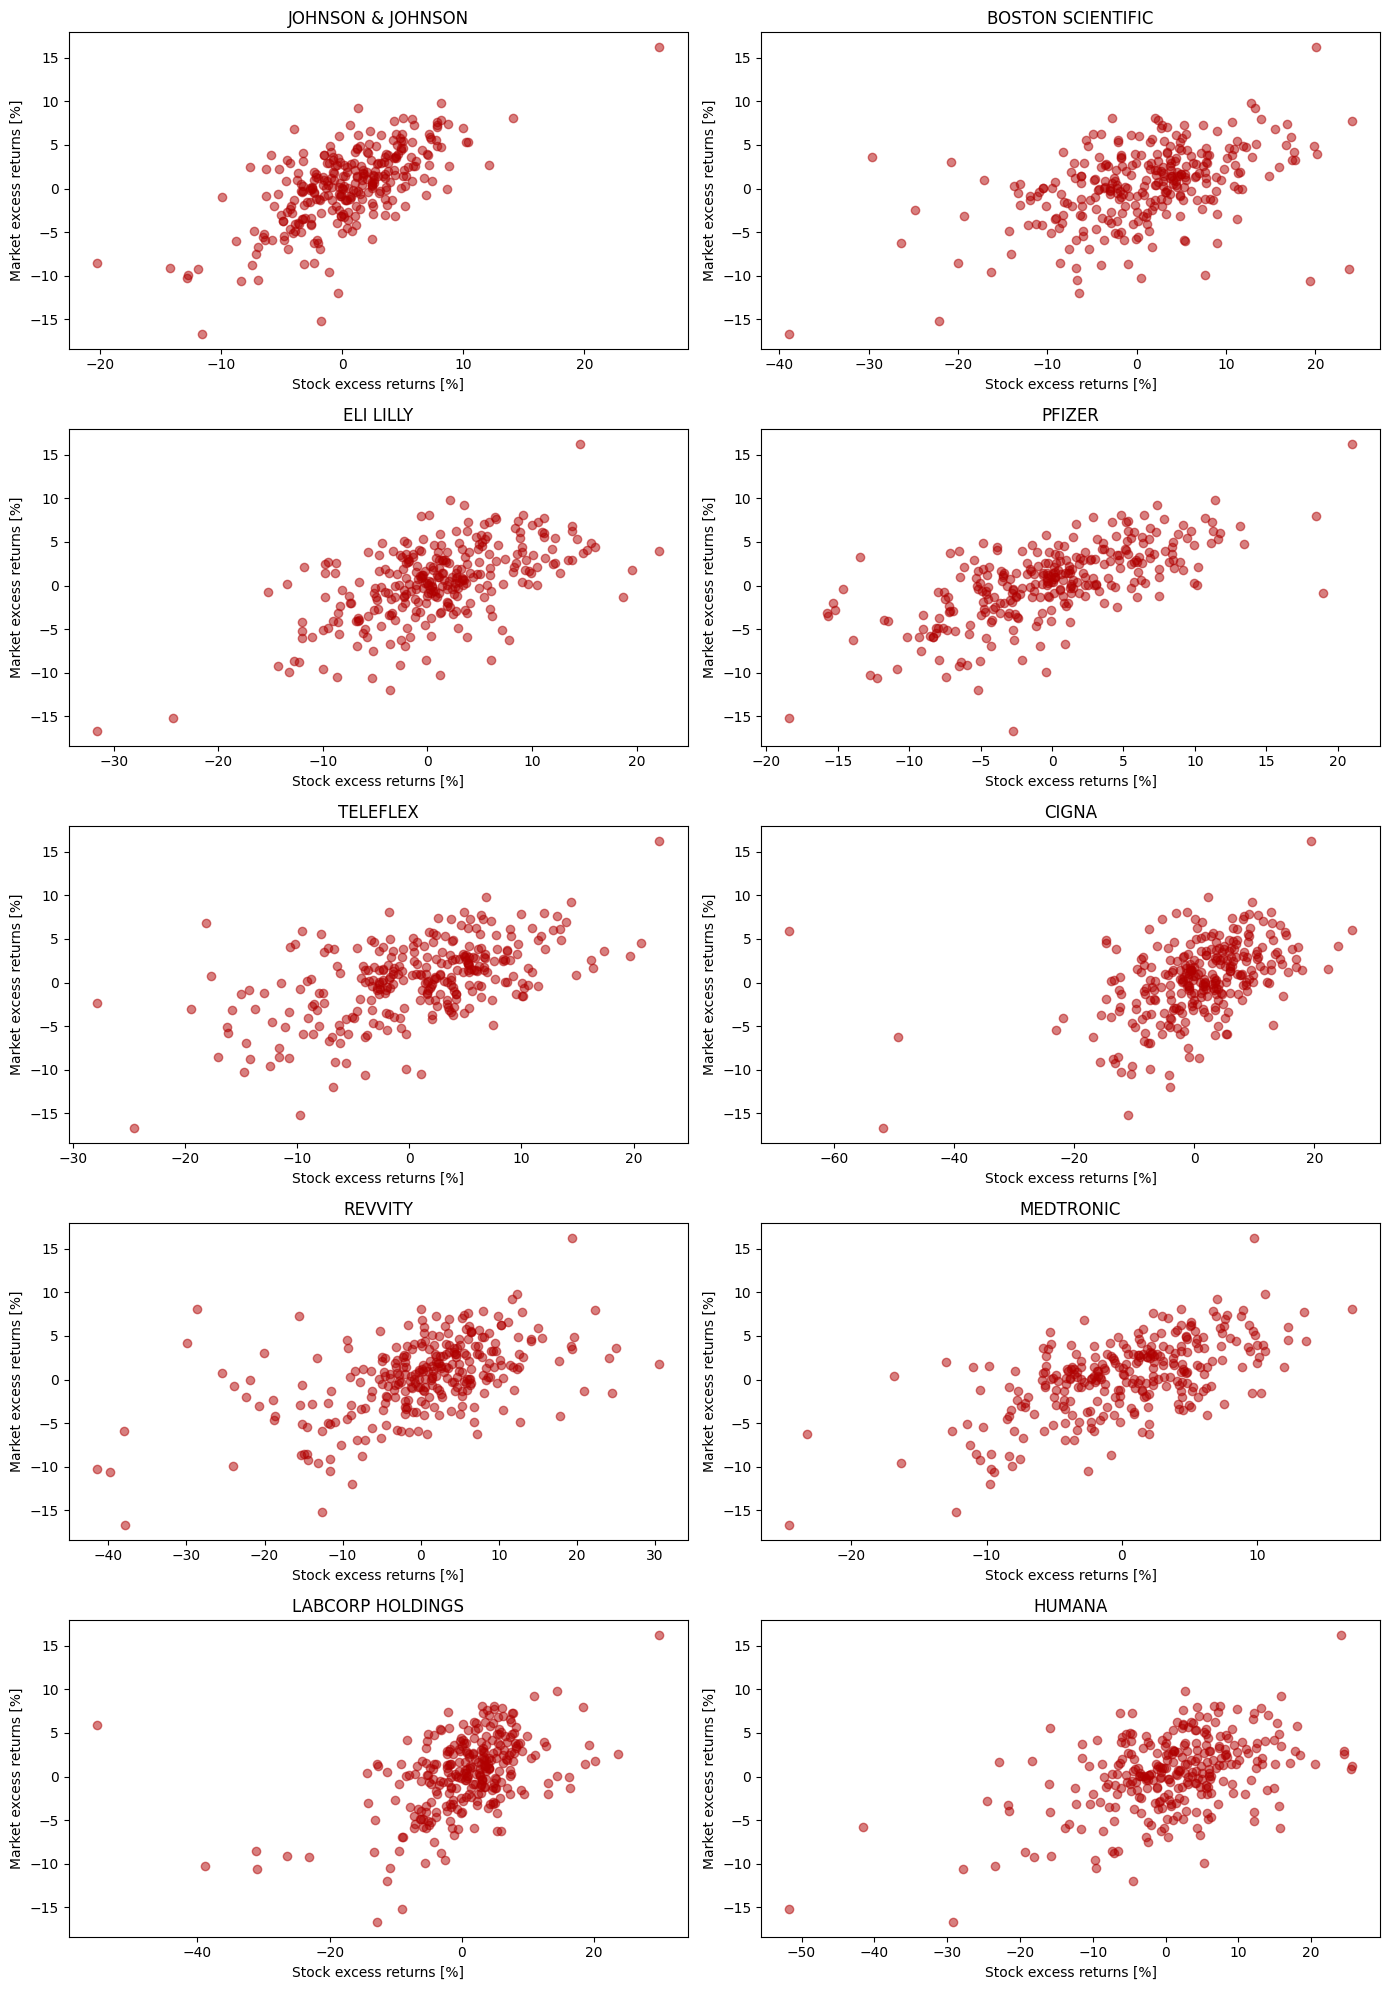
\includegraphics[width=0.8\textwidth]{images/equities_scatterplot.png}
    \caption{Scatterplot of equities' returns against excess market returns, with linear regression.}\label{fig:gigascatter}
\end{figure}